
\documentclass[9pt]{IEEEtran}

% basic
\usepackage[slovene]{babel}
\usepackage{graphicx,epstopdf,fancyhdr,amsmath,amsthm,amssymb,url,array,textcomp,svg,listings,hyperref,xcolor,colortbl,float,gensymb,longtable,supertabular,multicol,placeins}
\usepackage{diagbox}
 % `sumniki' in names
\usepackage[utf8x]{inputenc}
\usepackage{multirow}
\usepackage{makecell}

 % search and copy for `sumniki'
\usepackage[T1]{fontenc}
\usepackage{lmodern}
\input{glyphtounicode}
\pdfgentounicode=1

% tidy figures
\graphicspath{{./figures/}}
\DeclareGraphicsExtensions{.pdf,.png,.jpg,.eps}

% correct bad hyphenation here
\hyphenation{op-tical net-works semi-conduc-tor trig-gs}

% ============================================================================================

\title{\vspace{0ex} %
% TITLE IN HERE:
Izločanje očesnih artefaktov z uporabo postopka
analize neodvisnih komponent (ANK)
\\ \large{Izpitna seminarska naloga}\\ \normalsize{Komunikacija človek-računalnik 2021/22, Fakulteta za računalništvo in informatiko, Univerza v Ljubljani}}
\author{ %
% AUTHOR IN HERE:
Žiga~Kleine
\vspace{-4.0ex}
}

% ============================================================================================

\begin{document}

\maketitle

\begin{abstract}

V poročilu bomo predstavili implementacijo in delovanje programa za izločevanje artefaktov, ki v EEG posnetkih nastanejo predvsem med utripanjem oči in predstavljajo neželen šum na omenjenih posnetkih. Problema smo se lotili z uporabo postopka analize neodvisnih komponent (ANK). Ta metoda naš vhodni EEG signal $X(n)$ dimenzije $N*M$ pretvori v signal neodvisnih komponent $Y(n)$ in mešalno matriko. Mešalno matriko in signal neodvisnih komponent algoritem ANK najde na podlagi vhodnega signala. Dobljeni signal $Y(N)$ je velikosti $N*M$ in predstavlja $N$ neodvisnih komponent vhodnega signala $X(x)$. Iz signala komponent lahko nato izločimo komponente, na katrih so razvidni artefakti. Enako storimo tudi za istoležne komponente matrike $W^{-1}$ . Okrnjen signal komponent nato pretvorimo nazaj v vhodni signal, tokrat z odstranjenimi artefakti. Na koncu algoritem evaluiramo tako, da signal z odstranjenimi artefakti primerjamo z začetnim signalom.


\end{abstract}

\section{Uvod}

Implementacijo vmesnika, s katerim lahko s pomočjo možganske aktivnosti nadzorujemo računalnik, lahko razdelimo na 5 smiselnih faz. Te faze so: zajemanje signalov, preobdelava ali čiščenje signalov, izločanje značilk, klasifikacija in interakcija z računalnikom.

Pri tej seminarski nalogi smo se posvetili drugi prej omenjeni fazi, čiščenju signalov. Ko z elektrodami zajemamo električne signale na površini možganov, se v teh signalih zelo pogosto pojavljajo šumi, ki niso povezani z možgansko aktivnostjo. Te šume lahko razdelimo v štiri glavne kategorije: šume, ki jih povzroči EEG oprema, zunanje električne motnje, šume, ki jih povzročijo žice elektrod, in šume, ki jih povzroči subjekt ~\cite{gupta1996preprocessing}. Pri tej seminarski nalogi se bomo posvetili predvsem šumom, ki jih povzroči subjekt. Med najintenzivnejšimi šumi, še posebno pri elektrodah na sprednjem delu glave, so namreč šumi, ki jih povzročajo obrazne mišice med mežikanjem in premikanjem oči. Te bomo poskušali iz signala izločiti z metodo, ki izkoristi metodo analize neodvisnih komponent, da naš vhodni EEG signal pretvori v prostor $N$ neodvisnih komponent, v katerem lahko nato lažje najdemo in izločimo očesne artefakte.


\section{Metode}

Najprej bomo predstavili tehnično ozadje problema, nato pa bomo to znanje prestavili v prakso in predstavili še implementacijo samega programa. Program za izločanje očesnih artefaktov z uporabo postopka s analize neodvisnih komponent smo implementirali v programskem jeziku MATLAB.

\subsection{Tehnično ozadje}

\subsubsection{Prostorski filtri}

Prostorski filtri \ref{fig_1} so tipi filtrov, ki večkratni signal $X(n)$, sestavljen iz $N$ kanalov, transformirajo v prostor komponent, predstavljen s signalom $Y(n)$, s pomočjo linearne transformacije, podane v obliki mešalne matrike $W$ \ref{fig_1}.

Celotno transformacijo lahko torej zapišemo v obliki \ref{eq1}. V praksi sta $X(n)$ in $Y(n)$ večdimenzionalna signala, predstavljena z matrikami velikosti $N*M$, kjer $N$ predstavlja število signalov, $M$ pa dolžino vsakega signala, $W$ pa je matrika velikosti $N*N$. Ker gre za linearno preslikavo, lahko prostorski filter tudi obrnemo, in sicer tako, da poiščemo inverz matrike $W$, $W^{-1}$. Enačba v obratno smer je torej oblike \ref{eq2}. 

\begin{equation} \label{eq1}
Y(n) = WX(n)
\end{equation}

\begin{equation} \label{eq2}
\tilde{X}(n) = W^{-1}Y(n)
\end{equation}


\begin{figure}[!htb]
\centering
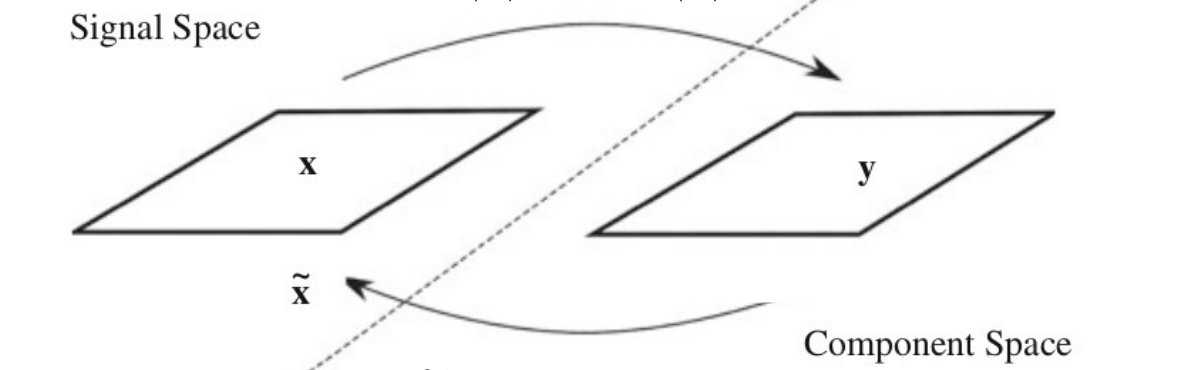
\includegraphics[width=1\columnwidth]{spatial_filter.png}
\caption[c1]{ Shema preslikave prostorskega filtra. }
\label{fig_1}
\end{figure}

Poznamo več vrst prostorskih filtrov, ki pretvarjajo vhodni signal v prostor komponent. Poznamo skupno srednjo referenco, bipolarno masko, prostorski odvod drugega reda, analizo neodvisnih komponent, analizo principalnih komponent, skupne prostorske vzorce ipd. V tej seminarski nalogi se bomo posvetili prostorskemu filtru z analizo neodvisnih komponent.

\subsubsection{Analiza neodvisnih komponent}

Metoda analize neodvisnih komponent (ANK) je relativno nova metoda za separacijo signalov, ki je na mnogo področjih pokazala boljše rezultate kot morda nekoliko bolj poznana metoda analize glavnih komponent. Eden izmed teh problemov je problem ekstrakcije in eliminacije očesnih artefaktov iz EEG signalov \cite{ochoa2002eeg}.

Metoda ANK  predpostavi, da je signal $X(n)$ mešanica $N$ neodvisnih izvornih signalov, ki jih lahko označimo z $S(x)$. Potem obstaja tudi časovno invariantna mešalna matrika $A$, ki signale $S(n)$ pretvori v signale $X(n)$ s pomočjo enačbe \ref{eq3}. Ker pa vemo, da velja tudi \ref{eq2}, lahko trdimo, da je $A \approx W^{-1}$. Iz dosedanjih podatkov lahko torej rečemo, da velja \ref{eq4}. 

S pomočjo postopka analize neodvisnih komponent lahko torej iz našega premešanega signala  $X(n)$  poskusimo predvideti matriki $A$ in $S(n)$, na podlagi katerih lahko nato dobimo približek signala v prostoru neodvisnih komponent, $Y(n)$.


\begin{equation} \label{eq3}
X(n) = AS(n)
\end{equation}

\begin{equation} \label{eq4}
Y(n) = WX(n) = WAS(n) \approx S(n)
\end{equation}

Dekomozicija na neodvisne komponente je mogoča, če vemo:

\begin{itemize}
  \item Da so signali $S(n)$ medsebojno neodvisni.
  \item Da signali $S(n)$ niso distribuirani po Gaussu.
  \item Da je število neodvisnih komponent enako številu snemanih signalov.
\end{itemize}

Če vse zgornje trditve veljajo, lahko uporabimo kanonično korelacijsko metodo za izračun signala v prostoru komponent in njemu pripadajočo mešalno matriko.


\subsubsection{Izločanje komponent in rekonstrukcija signala}

Signal želimo imeti v prostoru komponent zaradi večih razlogov. V našem primeru želimo imeti pregled nad osnovnimi komponentami, ki sestavljajo naše možgansko valovanje, z namenom, da izločimo nepotrebne šume.

Ko smo s pomočjo metode ANK dobili matriko v prostoru neodvisnih komponent $Y(n)$ in mešalno matriko $W^{-1}$, lahko v prostoru komponent izberemo le $P$ relevantnih komponent, tako, da iz stolpcev $W^{-1}$ in istoležnih vrstic $Y(n)$ izločimo vse šumne komponente. Tako dobimo novo matriko $Y(n)$ dimenzij $P*M$ in novo matriko  $W^{-1}$ dimenzij $N*P$. Če matriki zmnožimo, dobimo po formuli \ref{eq2} približek vhodnega signala $\tilde{X}(n)$, ki ne vsebuje izločenih komponent. Na tak način lahko iz signala izločimo komponente, ki vsebujejo neželene artefakte. 


% \begin{figure}[!htb]
% \centering
% 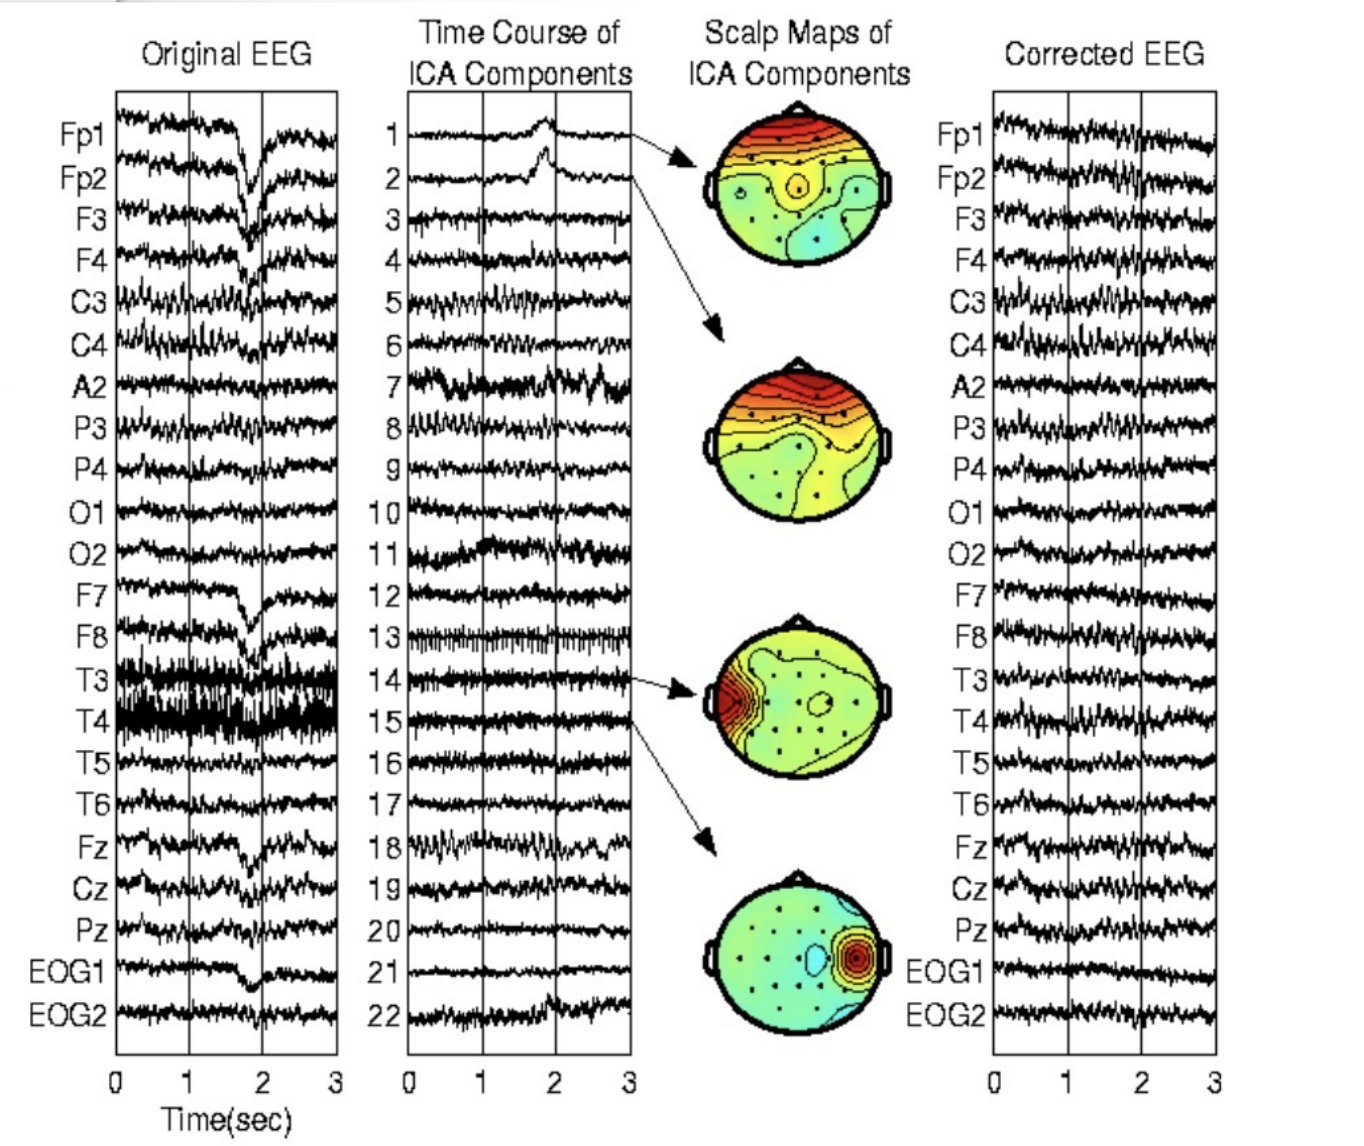
\includegraphics[width=1\columnwidth]{artefact_elimination.png}
% \caption[c1]{ Izločanje artefaktov. }
% \label{fig_2}
% \end{figure}


\subsection{Implementacija}

\subsubsection{Priprava signalov}

Signale smo pridobili iz opdprte podatkovne baze biomedicinskih signalov Physionet, specifično iz podatkovne baze EEG posnetkov z imenom EEG Motor Movement/Imagery Dataset (okrajšano eegmmidb) \cite{goldberger2000physiobank, schalk2004bci2000}. Pri procesiranju signalov smo si pomagali s programskim paketom wfdb, ki je na voljo tudi v programskem okolju MATLAB. Vsak izmed posnetkov v eegmmidb je nekajminutni signal 64-ih elekrod, nameščenih po glavi subjekta, ko subjekt opravlja različne naloge (mirovanje, stiskanje pesti, razmišljanje o stiskanju pesti). Signal smo v okolje prebrali s pomočjo funkcije, imenovane $rdsamp()$ iz programskega paketa wfdb.

\subsubsection{Analiza neodvisnih komponent}

Nad našim 64-kanalnim vhodnim signalom smo najprej naredili analizo neodvisnih komponent. Pomagali smo si s klicem funkcije $fastica()$, ki vhodni signal razdeli na signal 64 neodvisnih komponent $Y(n)$, na mešalno matriko  $W$ in na njen inverz $W^{-1}$.

\subsubsection{Topografski izris stolpcev matrike $W^{-1}$}

Stolpci matrike $W^{-1}$ nam lahko veliko povedo o posameznih komponentah v našem prostoru komponent, saj nam lahko povedo, na katerih elektrodah glave je omenjena komponenta najbolj in najmanj izrazita. Tu smo si pomagali s funkcijo $plot_topography()$, ki nam je topografsko vizualizirala vpliv vsake komponente na različne predele glave. Na podlagi teh vizualizacij smo nato ocenili, katere komponente so ekskluzivno zelo izrazite okoli predela oči, in jih izločili iz stolpcev matrike  $W^{-1}$ in istoležnih vrstic $Y(n)$.

\subsubsection{Izločanje artefaktov}

Ko smo ročno določili, katere komponente želimo iz signala izločiti, smo okrnjeni matriki $W^{-1}$ in $Y(n)$ zmnožili po formuli \ref{eq2}, in dobili nazaj korigiran EEG signal, tokrat brez neželenih artefaktov. 

\section{Rezultati}

V rezultatih bomo evaluirali implementirano metodo eliminacije artefaktov na signalu iz eegmmidb z imenom $S001R03.edf$. Kot smo že večkrat omenili, smo signal najprej razbili na signal v prostoru komponent in na mešalno matriko. Nato smo iz dobljenih matrik eliminirali komponente, za katere smo ocenili, da predstavljajo očesne artefakte. Odločili smo se eliminirati signale 2, 3, 17, 19, 24, 28, 34 in 46. Vhodni signal smo nato z okrnjenimi matrikami rekonstruirali.

Na slikah \ref{fig_7, fig_8} vidimo primera vizualizacij topografije stolpcev matrike $W^{-1}$. Na  prvi izmed slik \ref{fig_7} vidimo 3 primere komponent, ki smo jih izločili iz signala, na drugi  \ref{fig_8} pa 3 primere komponent, ki smo jih obdžali.


\begin{figure}[!htb]
\centering
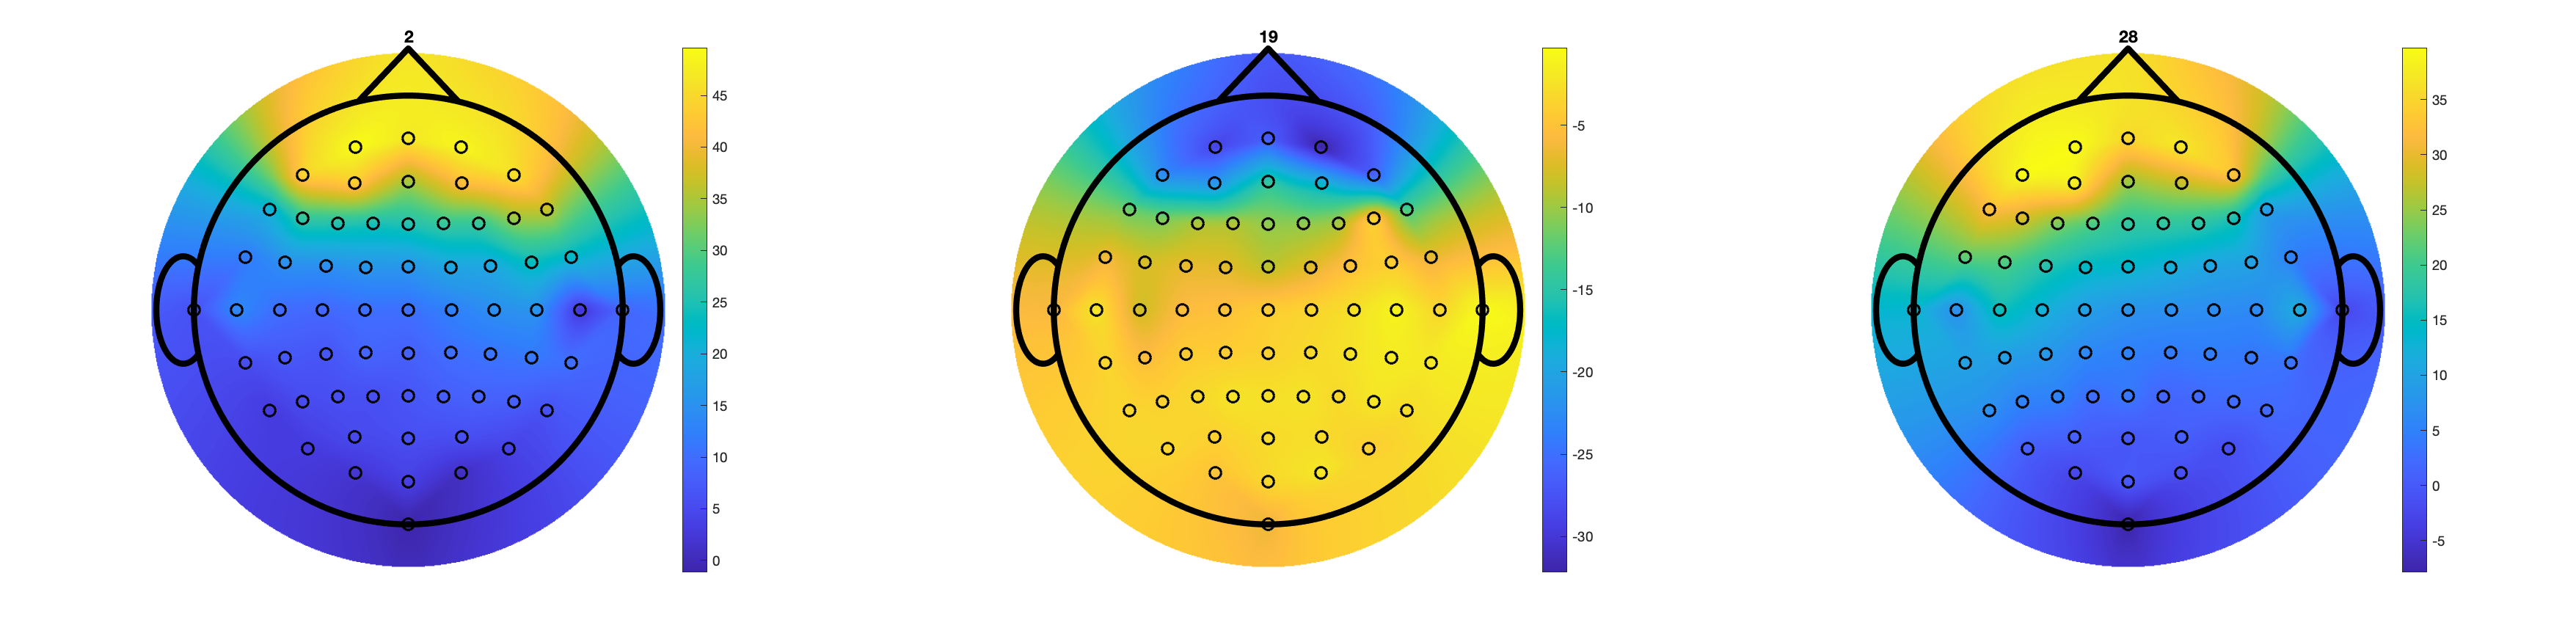
\includegraphics[width=1\columnwidth]{sigs_to_eliminate.png}
\caption[c1]{ Primeri topografije  komponent, ki jih želimo eliminirati.  }
\label{fig_7}
\end{figure}

\begin{figure}[!htb]
\centering
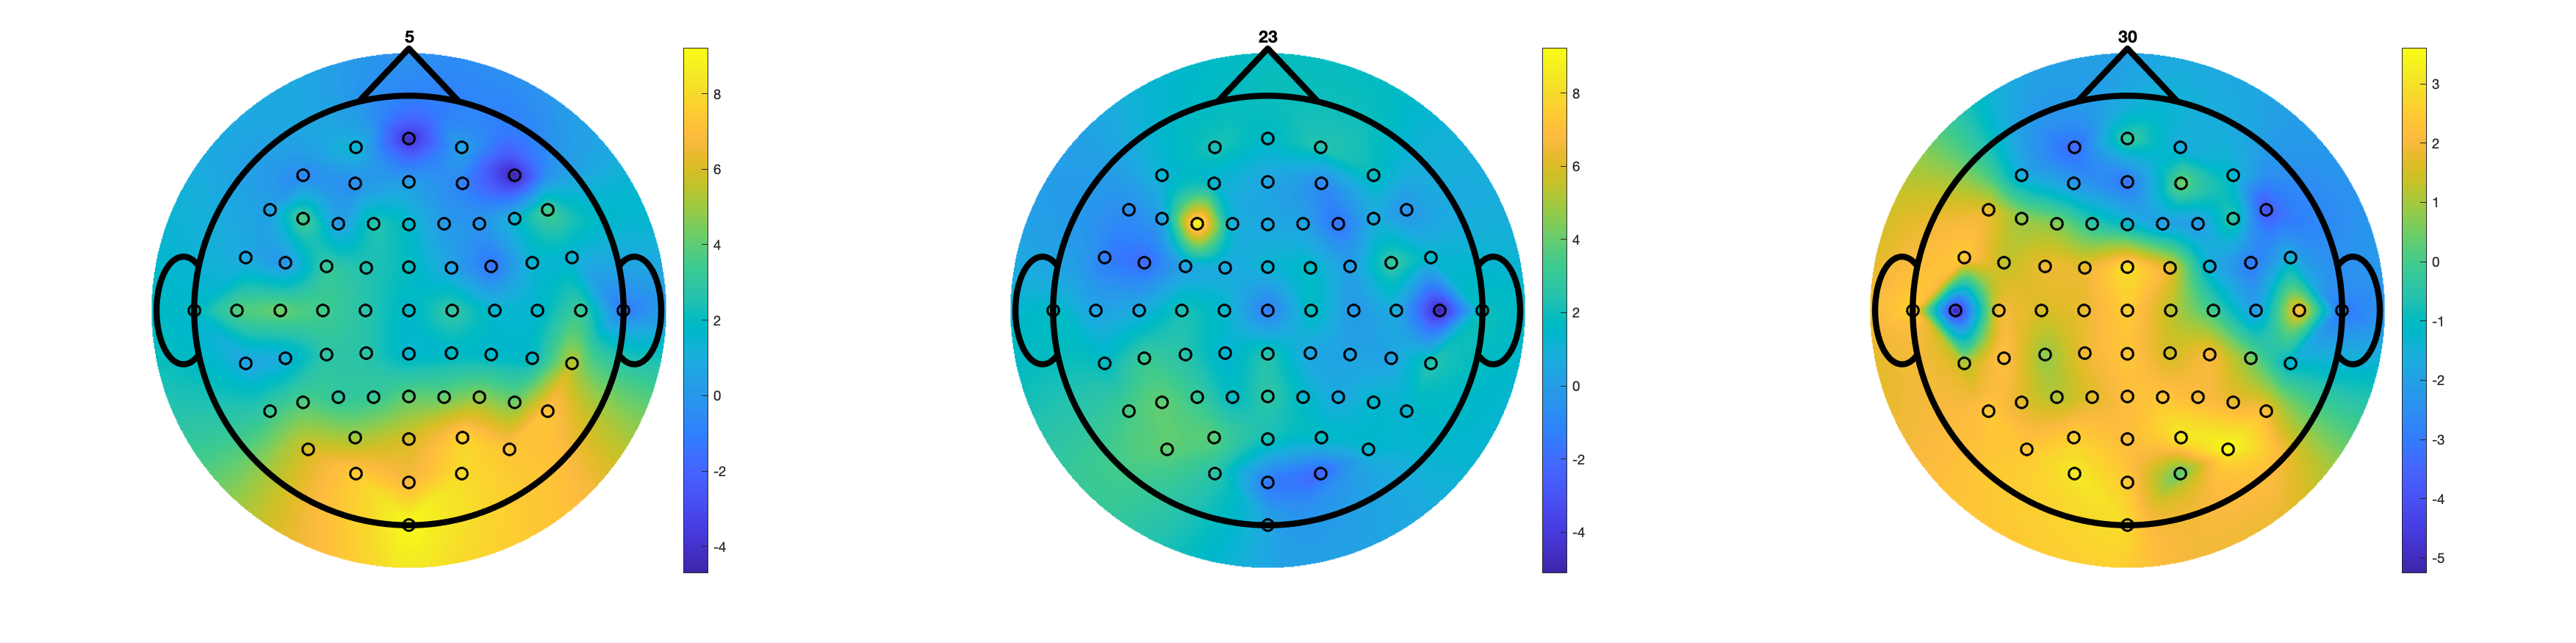
\includegraphics[width=1\columnwidth]{sigs_to_keep.png}
\caption[c1]{ Primeri topografije komponent, ki jih želimo obdržati. }
\label{fig_8}
\end{figure}

Sledijo vizualicije vseh 64 signalov posnetka $S001R03.edf$, najprej pred obdelavo \ref{fig_3}, nato v prostoru komponent \ref{fig_9}, in nazadnje še po izločanju artefaktov \ref{fig_4}.

\begin{figure}[!htb]
\centering
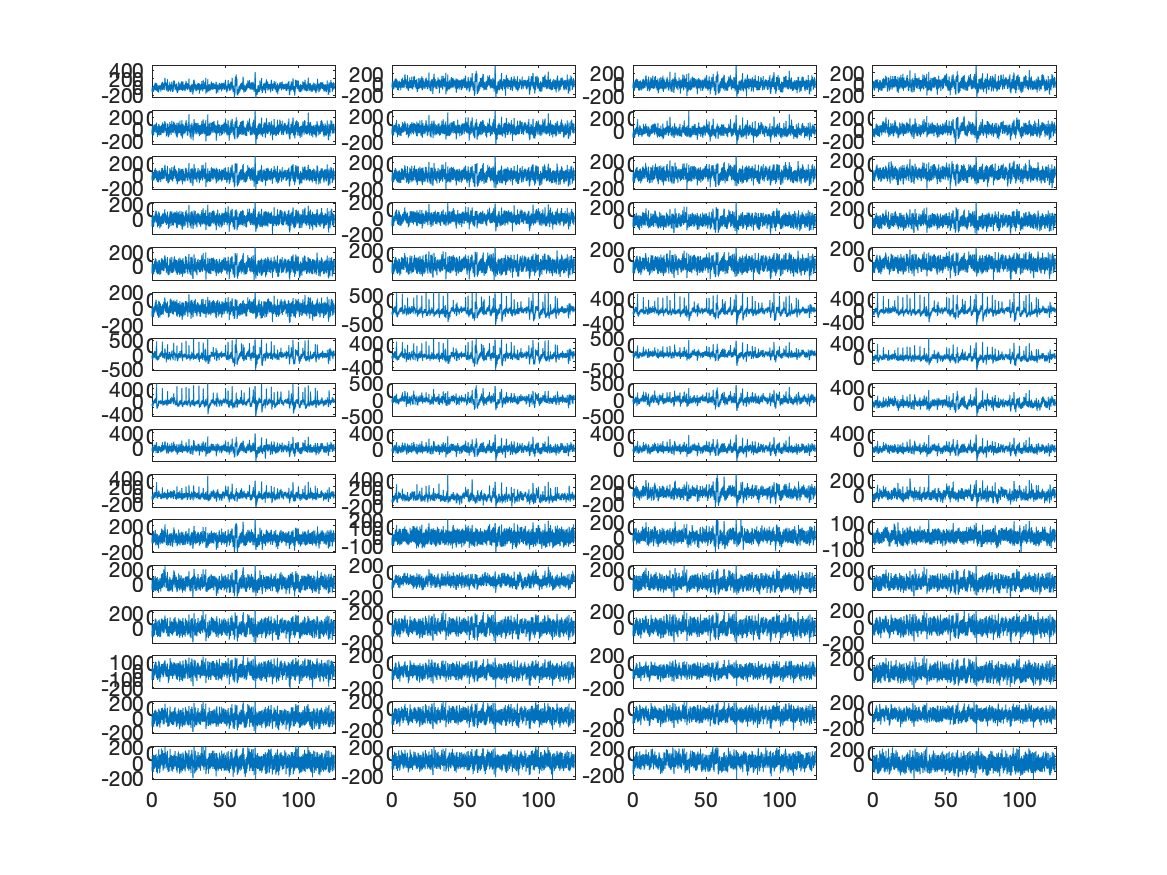
\includegraphics[width=1\columnwidth]{insig_all.png}
\caption[c1]{ Vsi signali posnetka $S001R03.edf$ pred odstranjevanjem artefaktov. }
\label{fig_3}
\end{figure}

\begin{figure}[!htb]
\centering
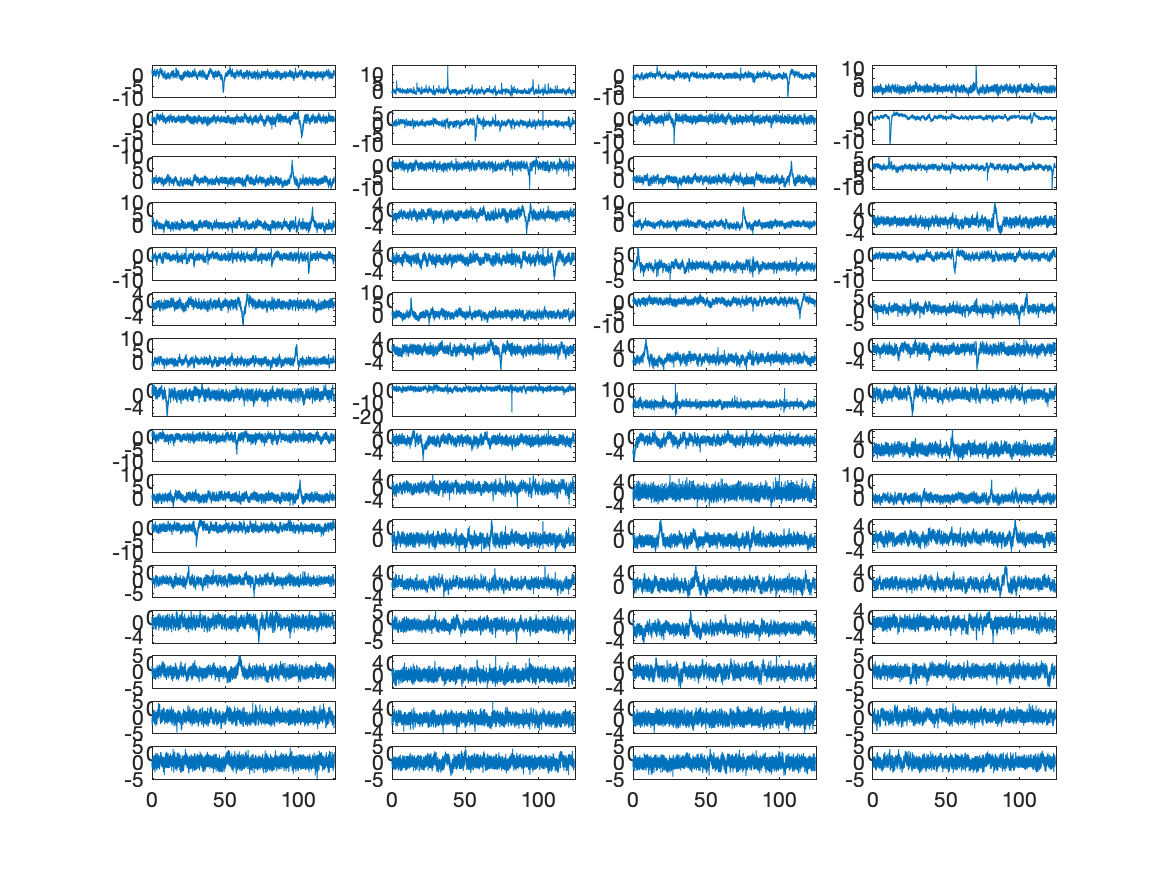
\includegraphics[width=1\columnwidth]{icasig_all.png}
\caption[c1]{ Vsi signali posnetka $S001R03.edf$ v prostoru komponent. }
\label{fig_9}
\end{figure}

\begin{figure}[!htb]
\centering
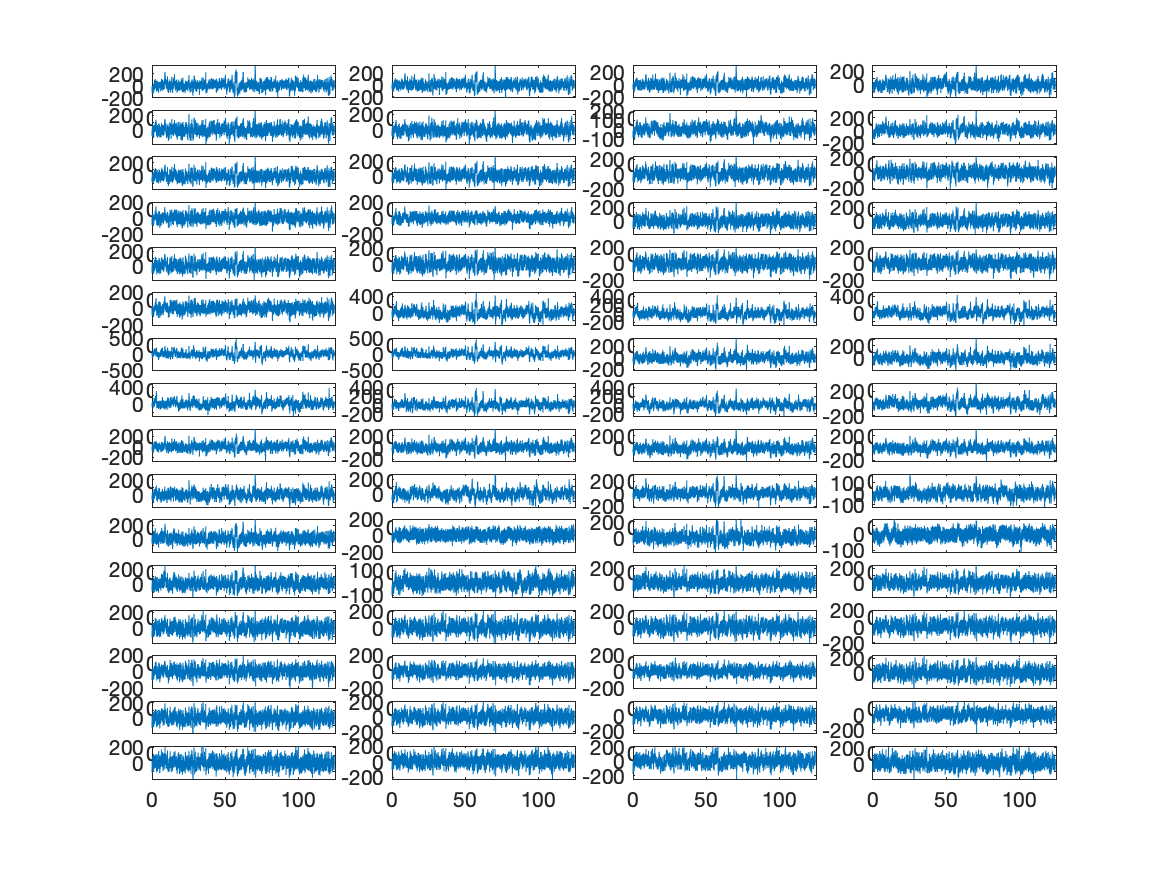
\includegraphics[width=1\columnwidth]{outsig_all.png}
\caption[c1]{ Vsi signali posnetka $S001R03.edf$ po odstranjevanju artefaktov. }
\label{fig_4}
\end{figure}

Ker je vizualizacija vseh 64 signalov iz posnetka nekoliko nepregledna, in iz njih na prvi pogled morda ni najbolje viden rezultat izločanja artefaktov, smo se odločili vizualizirati še odstranjevanje artefaktov na signalih, kjer so očesni artefakti najvidnejši. To sta signala elektrod $F_{P1}$ (22) \ref{fig_5} in $F_{P2}$ (24) \ref{fig_6}. Iz prikazanih vizualizicij lahko jasno vidimo, da so bili glavni vrhovi uspešno odstranjeni, brez da bi skrajšali sam signal, in s tem morda žrtvovali pomembne informacije, ki bi jih lahko izgubili, če bi vrhove preprosto izrezali iz signala.

\begin{figure}[!htb]
\centering
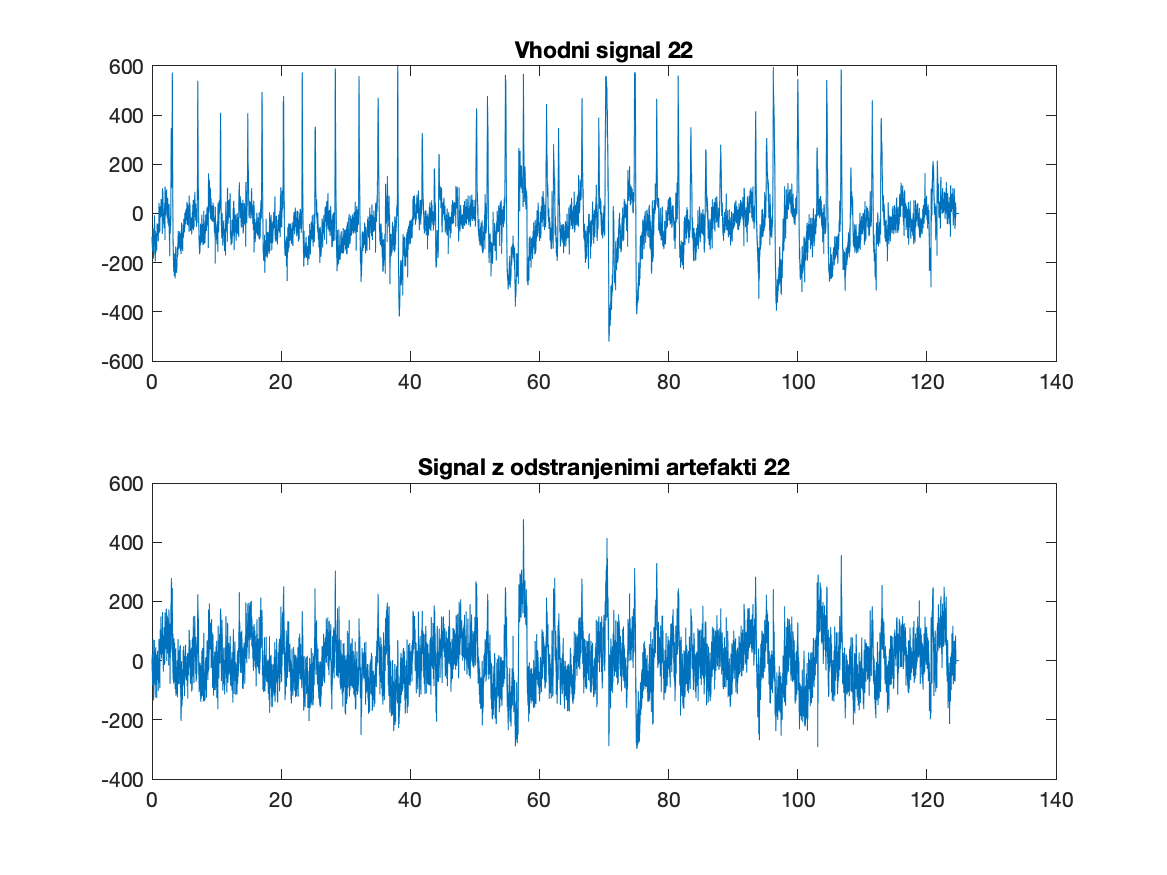
\includegraphics[width=1\columnwidth]{22_insig_outsig.png}
\caption[c1]{ Signal elektrode 22 z imenom $F_{P1}$ pred in po odstranjevanju artefaktov.  }
\label{fig_5}
\end{figure}

\begin{figure}[!htb]
\centering
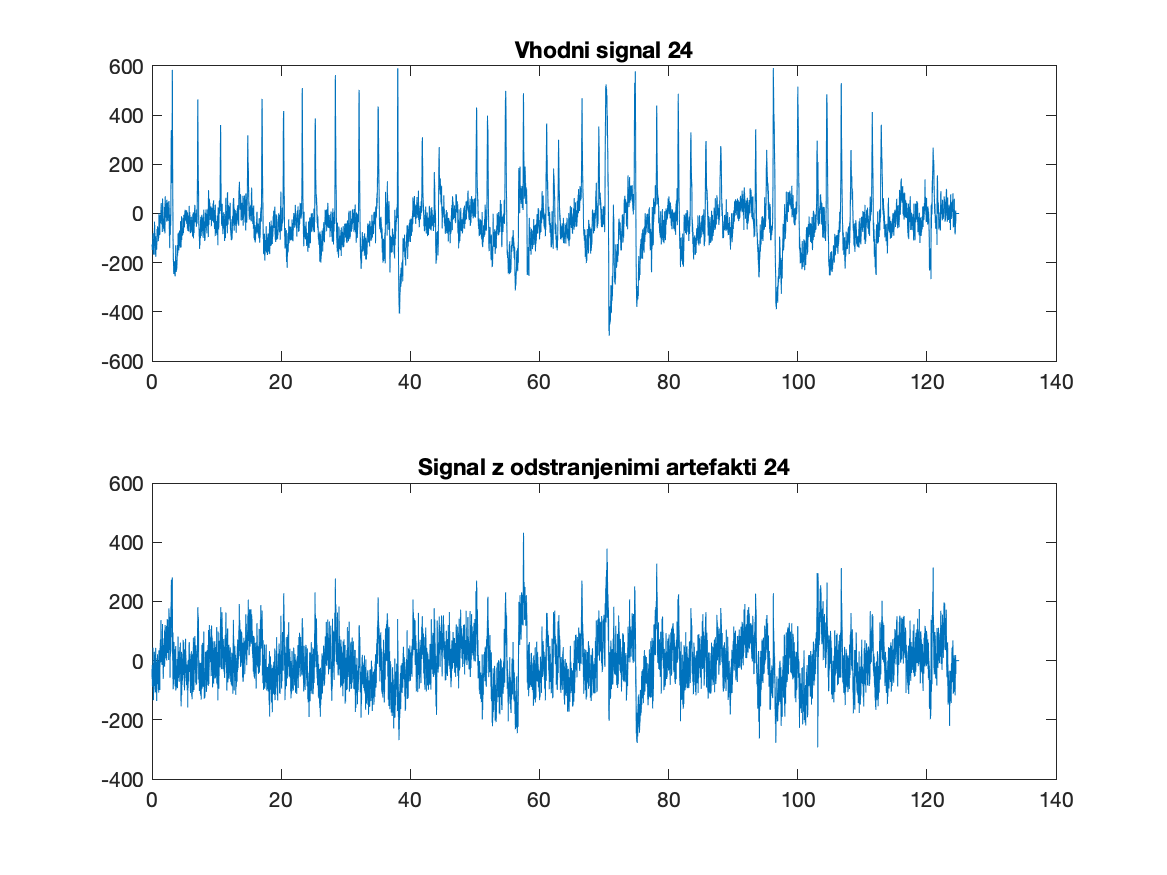
\includegraphics[width=1\columnwidth]{24_insig_outsig.png}
\caption[c1]{ Signal elektrode 24 z imenom $F_{P2}$ pred in po odstranjevanju artefaktov.}
\label{fig_6}
\end{figure}


\section{Diskusija}

Opisana metoda je precej učinkovita pri odstranjevanju artefaktov iz šumnih EEG signalov. Za razliko od pragovne metode nova metoda vrača izhodni signal, enako dolg kot vhodni signal, kar je prednost, saj smo s pragovno metodo pri pogostem mežikanju subjekta izgubili velik delež pomembnih informacij, ko smo izrezovali kose šumnega signala.

Potencialni problemi seveda nastanejo pri izločanju šumnih komponent. Kljub dobri topološki vizualizaciji mešalne matrike smo imeli z izločanjem potencialnih šumnih komponent kar nekaj težav. V teoriji smo namreč vedeli, da moramo izločiti komponente, ki močno vplivajo na signal elektrod v okolici oči. V praksi pa se je problem izkazal za nekoliko težjega, saj je bilo med komponentami več takih, ki so bile za naše laične oči dvoumne. Šum bi lahko bolje odstranili, če bi imeli pri izločanju šumnih komponent na voljo pomoč strokovnjaka. 

\bibliographystyle{IEEEtran}
\bibliography{bibliography}

\end{document}
